%% fig04-bilinear-weights, caption is in docs/figures/README.md
\documentclass[border=8pt]{standalone}
% Shared preamble for the interpolation-geometry figures.
% \input by every figNN-*.tex. 
\usepackage[T1]{fontenc}
\usepackage{amsmath,amssymb}
\usepackage{tikz}
\usetikzlibrary{shapes.misc,arrows.meta,calc,decorations.pathreplacing,positioning,fit,backgrounds}

\definecolor{ink}{HTML}{1A1A1A}
\definecolor{gridc}{HTML}{9AA3AD}
\definecolor{accent}{HTML}{1F5FA9}
\definecolor{good}{HTML}{2E7D4F}
\definecolor{bad}{HTML}{B03030}
\definecolor{soft}{HTML}{E6EDF7}
\definecolor{softg}{HTML}{E3F0E8}
\definecolor{softr}{HTML}{F8E6E6}
\definecolor{amber}{HTML}{B8860B}


\tikzset{
  gpt/.style={circle,fill=ink,inner sep=1.15pt},
  ghost/.style={circle,draw=gridc,fill=white,inner sep=1.15pt},
  dep/.style={cross out,draw=accent,thick,inner sep=1.6pt,minimum size=4pt},
  traj/.style={gridc,dotted,thick,-{Stealth[length=2mm]}},
  htraj/.style={accent,very thick,-{Stealth[length=2.6mm]}},
  lbl/.style={font=\footnotesize},
  slbl/.style={font=\scriptsize},
}

\begin{document}
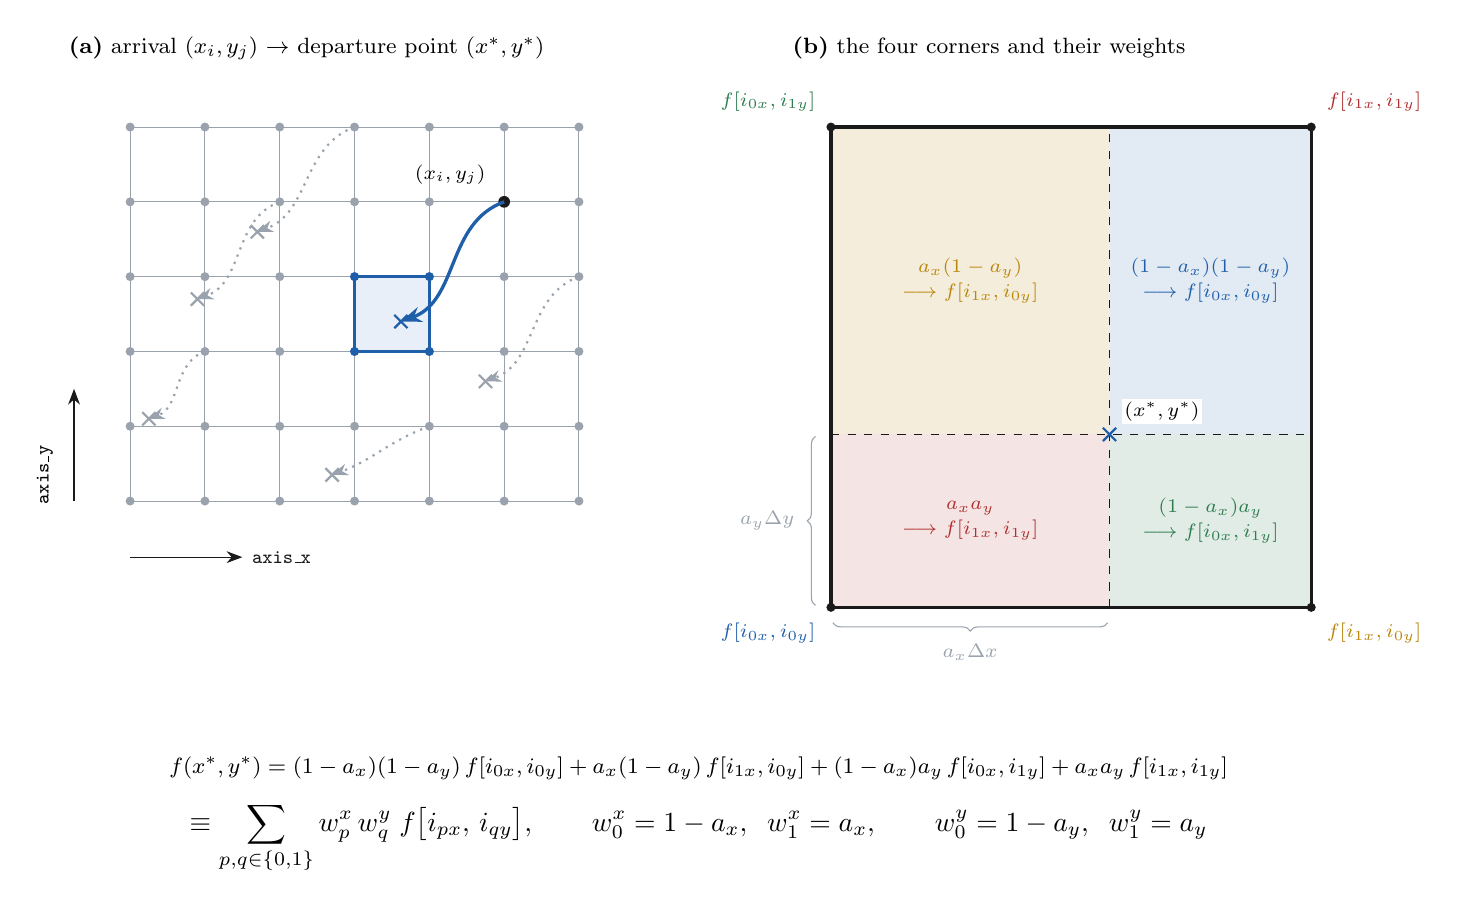
\begin{tikzpicture}[x=0.95cm,y=0.95cm]
  % ---------- (a) grid with trajectory ----------
  \begin{scope}[yshift=1.2cm]
    \node[lbl,anchor=west] at (-0.95,6.05) {\textbf{(a)} arrival $(x_i,y_j)$ $\to$ departure point $(x^{*},y^{*})$};
    \draw[gridc,thin] (0,0) grid[step=1] (6,5);
    \foreach \i in {0,...,6} \foreach \j in {0,...,5} \node[gpt,gridc] at (\i,\j) {};
    \fill[soft,opacity=0.9] (3,2) rectangle (4,3);
    \draw[accent,very thick] (3,2) rectangle (4,3);
    \foreach \p in {(3,2),(4,2),(3,3),(4,3)} \node[gpt,accent] at \p {};
    \foreach \a/\b/\c/\d in {2/4/0.9/2.7, 4/1/2.7/0.35, 1/2/0.25/1.1, 6/3/4.75/1.6, 3/5/1.7/3.6}{
      \draw[traj] (\a,\b) to[out=200,in=20] (\c,\d);
      \node[dep,gridc] at (\c,\d) {};
    }
    \node[circle,fill=ink,inner sep=1.5pt] at (5,4) {};
    \node[slbl,anchor=south east] at (4.88,4.10) {$(x_i,y_j)$};
    \draw[htraj] (5,4) to[out=200,in=20] (3.62,2.40);
    \node[dep] at (3.62,2.40) {};
    \draw[-{Stealth[length=2mm]},ink] (0,-0.75) -- (1.5,-0.75) node[slbl,anchor=west] {\texttt{axis\_x}};
    \draw[-{Stealth[length=2mm]},ink] (-0.75,0) -- (-0.75,1.5);
    \node[slbl,anchor=south,rotate=90] at (-0.9,0.35) {\texttt{axis\_y}};
  \end{scope}
  % ---------- (b) blow-up of the cell ----------
  \begin{scope}[xshift=8.9cm,yshift=-0.15cm,x=1.22cm,y=1.22cm]
    \pgfmathsetmacro{\S}{5}
    \pgfmathsetmacro{\ax}{0.58}
    \pgfmathsetmacro{\ay}{0.36}
    \pgfmathsetmacro{\fx}{\S*\ax}
    \pgfmathsetmacro{\fy}{\S*\ay}
    \node[lbl,anchor=west] at (-0.5,5.82) {\textbf{(b)} the four corners and their weights};
    \fill[bad,opacity=0.13]    (0,0)     rectangle (\fx,\fy);
    \fill[good,opacity=0.15]   (\fx,0)   rectangle (\S,\fy);
    \fill[amber,opacity=0.15]  (0,\fy)   rectangle (\fx,\S);
    \fill[accent,opacity=0.13] (\fx,\fy) rectangle (\S,\S);
    \draw[ink,very thick] (0,0) rectangle (\S,\S);
    \draw[ink,dashed] (\fx,0) -- (\fx,\S);
    \draw[ink,dashed] (0,\fy) -- (\S,\fy);
    \foreach \p in {(0,0),(\S,0),(0,\S),(\S,\S)} \node[gpt] at \p {};
    \node[slbl,accent,anchor=north east,align=right] at (-0.06,-0.06)
       {$f[i_{0x},i_{0y}]$};
    \node[slbl,amber,anchor=north west,align=left] at (\S+0.06,-0.06)
       {$f[i_{1x},i_{0y}]$};
    \node[slbl,good,anchor=south east,align=right] at (-0.06,\S+0.06)
       {$f[i_{0x},i_{1y}]$};
    \node[slbl,bad,anchor=south west,align=left] at (\S+0.06,\S+0.06)
       {$f[i_{1x},i_{1y}]$};
    \node[dep] at (\fx,\fy) {};
    \node[slbl,anchor=south west,fill=white,inner sep=1pt] at (\fx+0.12,\fy+0.1) {$(x^{*},y^{*})$};
    \node[slbl,accent,align=center] at ({(\fx+\S)/2},{(\fy+\S)/2})
       {$(1-a_x)(1-a_y)$\\[1pt]$\longrightarrow f[i_{0x},i_{0y}]$};
    \node[slbl,amber,align=center] at ({\fx/2},{(\fy+\S)/2})
       {$a_x(1-a_y)$\\[1pt]$\longrightarrow f[i_{1x},i_{0y}]$};
    \node[slbl,good,align=center] at ({(\fx+\S)/2},{\fy/2})
       {$(1-a_x)a_y$\\[1pt]$\longrightarrow f[i_{0x},i_{1y}]$};
    \node[slbl,bad,align=center] at ({\fx/2},{\fy/2})
       {$a_xa_y$\\[1pt]$\longrightarrow f[i_{1x},i_{1y}]$};
    \draw[decorate,decoration={brace,amplitude=3pt,mirror},gridc] (0.02,-0.16) -- (\fx-0.02,-0.16);
    \node[slbl,gridc,anchor=north] at ({\fx/2},-0.28) {$a_x\Delta x$};
    \draw[decorate,decoration={brace,amplitude=3pt},gridc] (-0.16,0.02) -- (-0.16,\fy-0.02);
    \node[slbl,gridc,anchor=east] at (-0.28,{\fy/2}) {$a_y\Delta y$};
  \end{scope}
  % ---------- the interpolant ----------
  \node[anchor=north,align=center,inner sep=0pt] at (7.6,-2.15)
  {\footnotesize
   $\displaystyle f(x^{*},y^{*})=(1-a_x)(1-a_y)\,f[i_{0x},i_{0y}]
    +a_x(1-a_y)\,f[i_{1x},i_{0y}]
    +(1-a_x)a_y\,f[i_{0x},i_{1y}]
    +a_xa_y\,f[i_{1x},i_{1y}]$\\[7pt]
   $\displaystyle \equiv\sum_{p,q\in\{0,1\}} w^x_p\,w^y_q\;f\big[i_{px},\,i_{qy}\big],
    \qquad w^x_0=1-a_x,\;\; w^x_1=a_x,\qquad w^y_0=1-a_y,\;\; w^y_1=a_y$};
\end{tikzpicture}
\end{document}
